\section{Demo details}
\label{sec:demo}

\begin{figure}
\centering
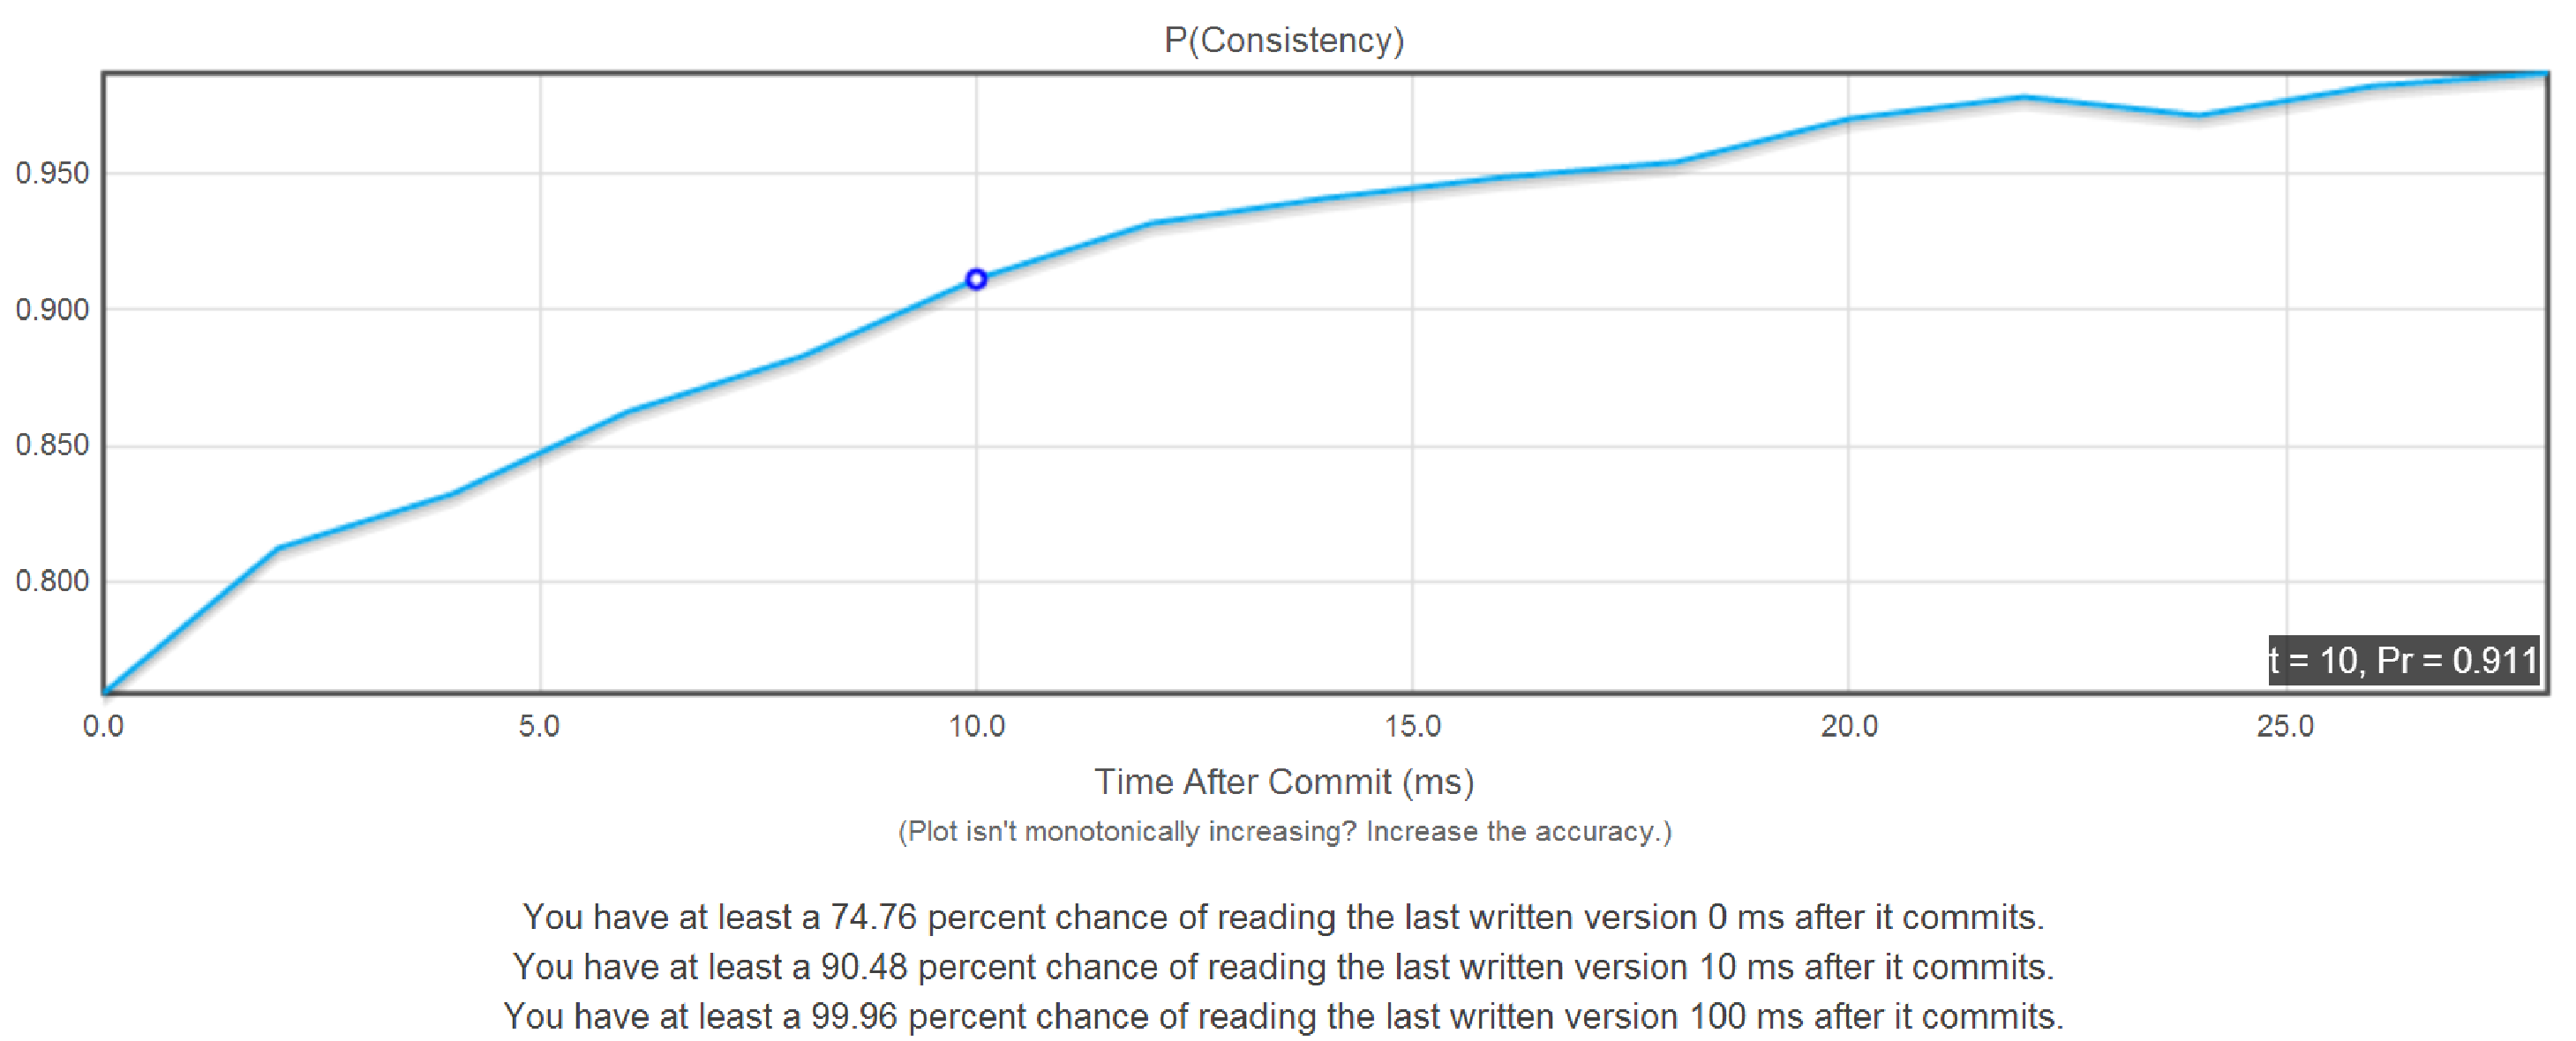
\includegraphics[width=.90\columnwidth]{figs/pbs-demo-screenshot.pdf}
\caption{A screenshot of a PBS demo indicating the values of t-visibility for a
given latency distribution. Our admin interface will be an extension of this
demo and will highlight the observed consistency measurements.}
\label{fig:pbs-demo-screenshot}
\end{figure}


%Overall theme of the demo and what are goals are: Showing how PBS-metrics can be
%integrated into the DB admin's interface. Also showing why consistency metrics
%are important and how PBS can be used to measure this etc.

\subsection{Demo Setup}
We will present an end-to-end demonstration that will show how metrics defined
by PBS can be used to capture the impact of consistency on user experience. We
will also highlight how database administrators can monitor and modify system
parameters to trade-off consistency for latency. The demonstration will consist
of the following components:\\

%Specific demo setup details: What is the app going to be -- What tables is it
%going to contain and how is this stored in Cassandra ?

\textbf{Web Application:} We will be using a hosted Twitter-like application. We
plan to make a web-interface that will be available to all SIGMOD attendees and
a mobile application that can be used to post messages about the conference.\\

\textbf{Distributed Datastore:} We plan to host a 50-node Cassandra cluster on
EC2 to support our web application. The Cassandra instances will use a table to
store the tweets published and a separate table to store the follower/following
relationship information.\\

\textbf{Data Sets:} In addition to the tweets posted by SIGMOD attendees, we
plan to inject the datastore with a corpus of 936,236 conversations obtained
from a crawl between Feb and July 2011. This will help us explore some of the
issues which arise with a heavier workload.

%Demo screens detail - We will have two screens and what each one will show. How
%can the audience interact with the demo ?
\subsection{Demo Interactions}

We plan to have two screens setup during the demo session: the first screen will
show the database administrator's interface, while the second one will be used
to show the user-interface for our web application. \\

\textbf{DB admin interface:} We plan to show a monitoring console that
measures and plots the consistency and latency over 10-second time intervals.
Additionally the admin interface will allow users to modify system parameters
like the replication factor and also set consistency SLAs for read and write
operations. Figure~\ref{fig:pbs-demo-screenshot} shows an example of how our 
dashboards will look. \\

\textbf{User-interface:} The user-interface screen will be show our
web-application described previously and will allow attendees to post and read
tweets. As these tweets are submitted to our Cassandra cluster, attendees can
witness how user-visible latency and consistency are captured in the monitoring
interface. 

%What are the scenarios that we will demonstrate / highlight ? Talk about chaos
%console to inject failure, delays and check how this affects consistency etc.
\subsection{Demo Scenarios}
We plan to explore many different scenarios to demonstrate how the latency
consistency trade-off is affected by changes to environment in which the
datastore is hosted. We will be hosting a \textit{chaos console} that can be
used to inject message delays, model messages being dropped and finally even
kill Cassandra instances randomly to see its effect on consistency. We believe
that this will highlight the importance of consistency prediction in datacenter
environments where such failures could occur frequently.
